\chapter{Further results}
\label{app:results}

\section{Initialization}
\label{app:sec:initialization}

This section provides examples of NCA projections on various data sets using different initializations. This is particularly useful to contrast the importance of initializations. Also it shows how NCA typically performs on small sized data sets. 

% The objective function is maximized using conjugate gradients and the entire data sets are used for training. Data sets used are: \texttt{iris}, \texttt{balance} and \texttt{ecoli}. Data set characteristics were presented before in Table, Chapter \ref{ch:evaluation}. 

\begin{figure}
	  \centering
	  \subfigure[NCA projection after random initialization]{\label{fig:iris-init-2}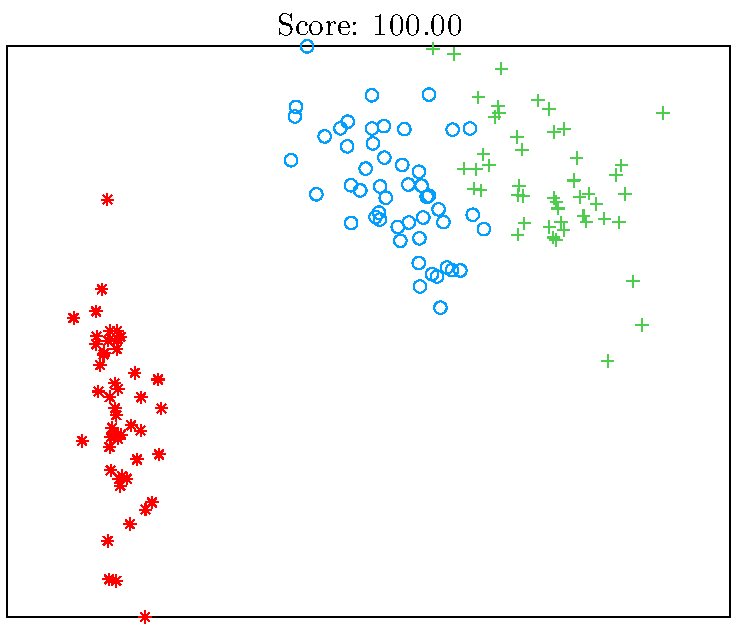
\includegraphics[width=0.47\textwidth]{images/iris-init-2}}
	  \subfigure[NCA projection after PCA initialization]{\label{fig:iris-init-4}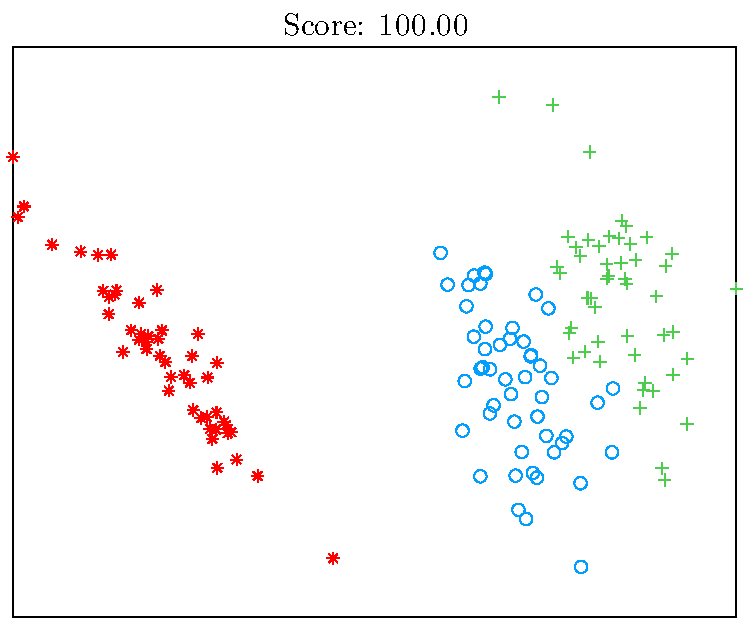
\includegraphics[width=0.47\textwidth]{images/iris-init-4}}
	  \subfigure[NCA projection after LDA initialization]{\label{fig:iris-init-6}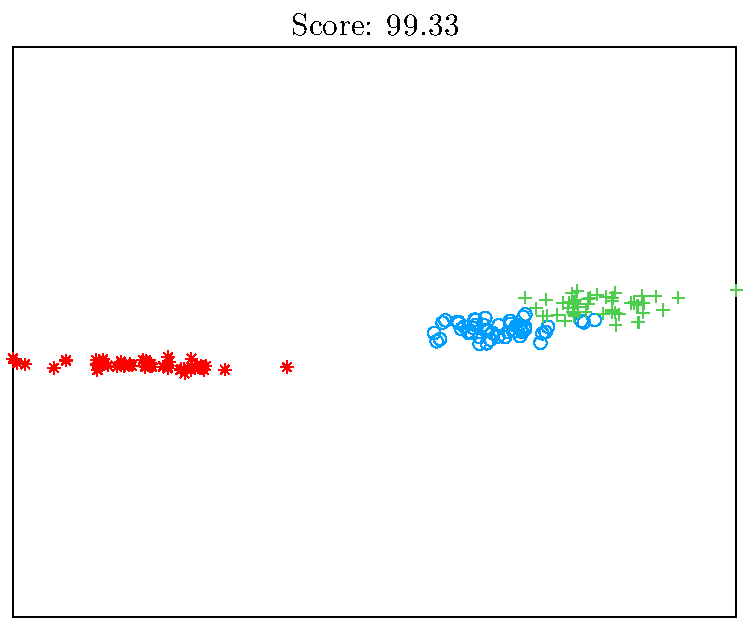
\includegraphics[width=0.47\textwidth]{images/iris-init-6}}
	  \subfigure[NCA projection after RCA initialization]{\label{fig:iris-init-8}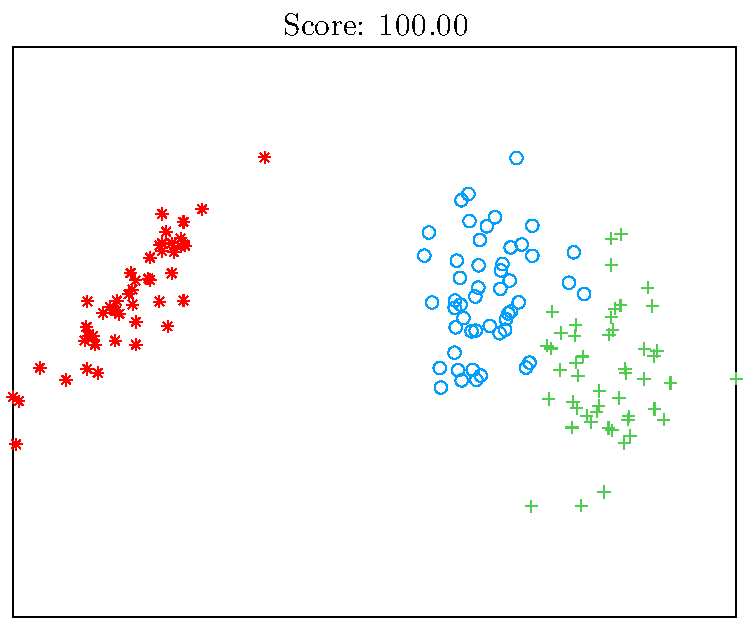
\includegraphics[width=0.47\textwidth]{images/iris-init-8}}
	  \caption{\small Results on \texttt{iris} data set.}
	  \label{fig:iris-init}
\end{figure}

\begin{figure}
	  \centering
	  \subfigure[NCA projection after random initialization]{\label{fig:balance-init-2}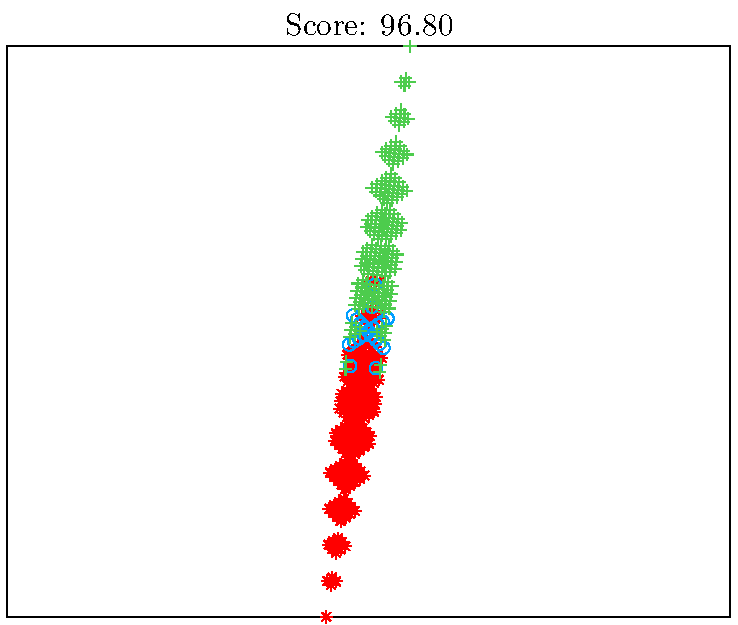
\includegraphics[width=0.47\textwidth]{images/balance-init-2}}
	  \subfigure[NCA projection after PCA initialization]{\label{fig:balance-init-4}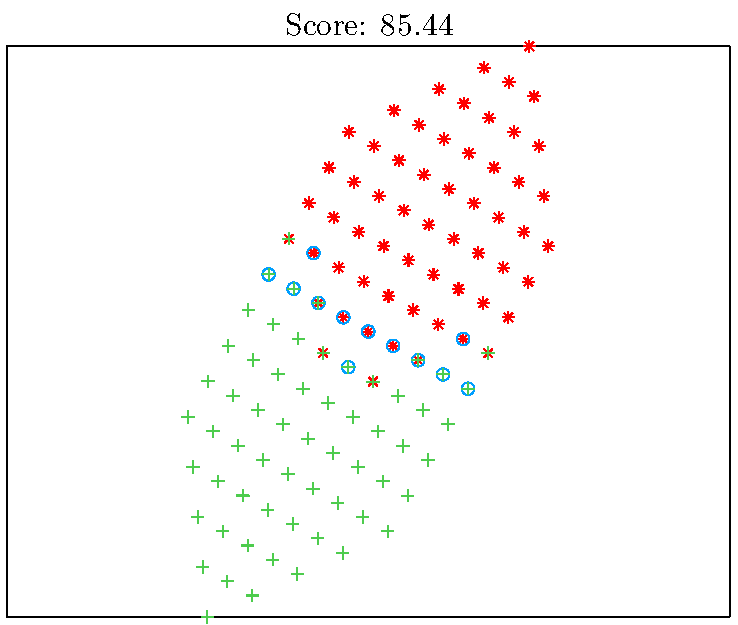
\includegraphics[width=0.47\textwidth]{images/balance-init-4}}
	  \subfigure[NCA projection after LDA initialization]{\label{fig:balance-init-6}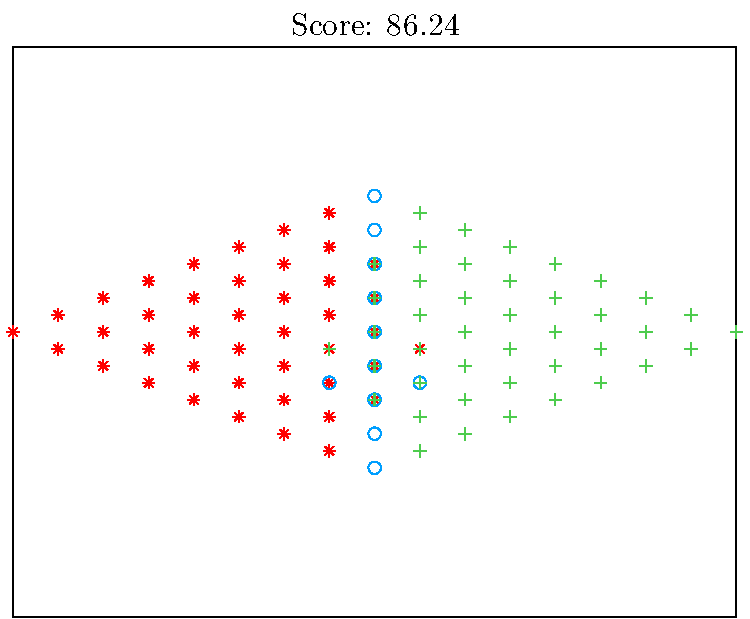
\includegraphics[width=0.47\textwidth]{images/balance-init-6}}
	  \subfigure[NCA projection after RCA initialization]{\label{fig:balance-init-8}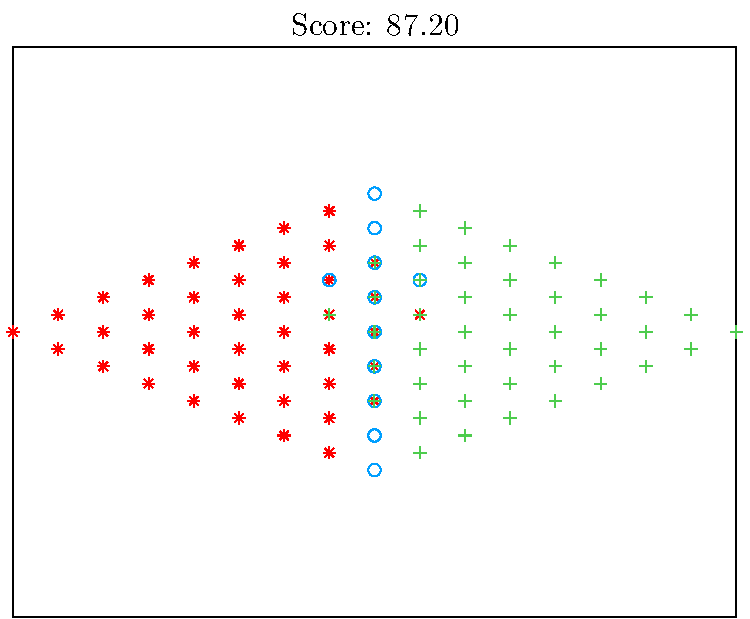
\includegraphics[width=0.47\textwidth]{images/balance-init-8}}
	  \caption{\small Results on \texttt{balance} data set.}
	  \label{fig:balance-init}
\end{figure}

\begin{figure}
	  \centering
	  \subfigure[NCA projection after random initialization]{\label{fig:ecoli-init-2}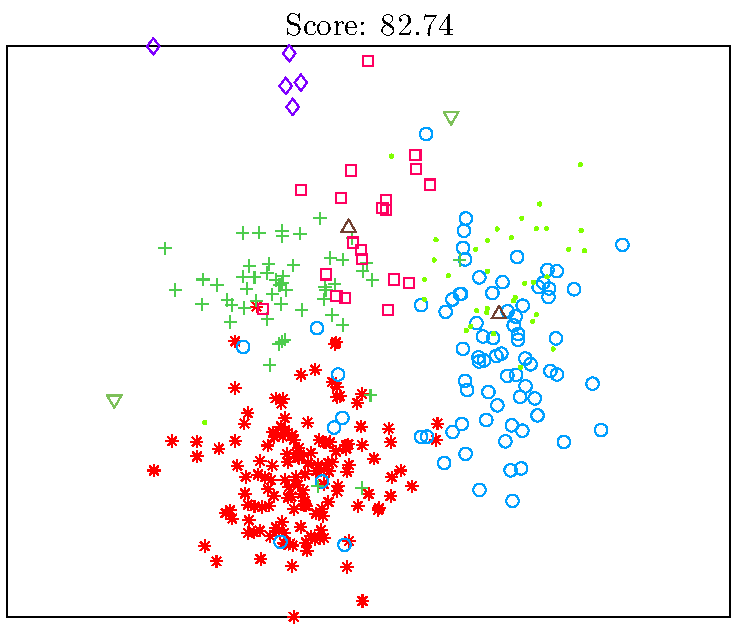
\includegraphics[width=0.47\textwidth]{images/ecoli-init-2}}
	  \subfigure[NCA projection after PCA initialization]{\label{fig:ecoli-init-4}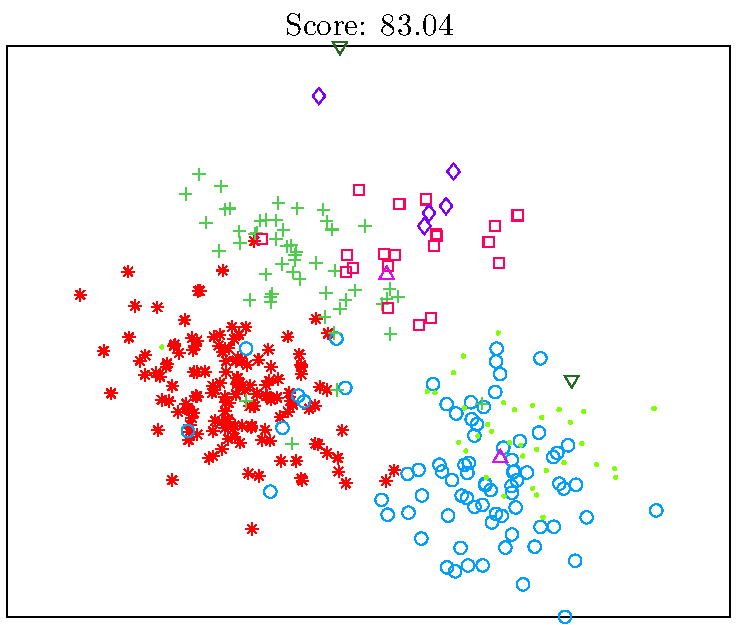
\includegraphics[width=0.47\textwidth]{images/ecoli-init-4}}
	  \subfigure[NCA projection after LDA initialization]{\label{fig:ecoli-init-6}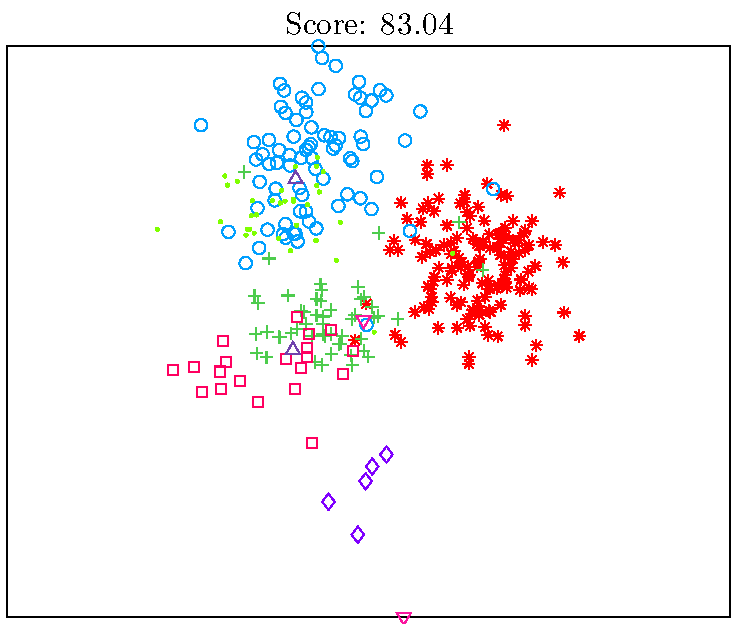
\includegraphics[width=0.47\textwidth]{images/ecoli-init-6}}
	  \subfigure[NCA projection after RCA initialization]{\label{fig:ecoli-init-8}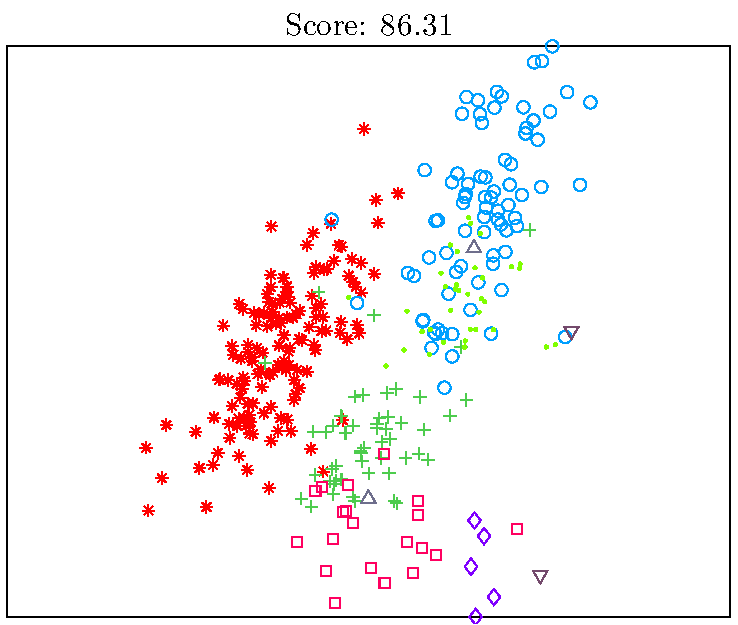
\includegraphics[width=0.47\textwidth]{images/ecoli-init-8}}
	  \caption{\small Results on \texttt{ecoli} data set.}
	  \label{fig:ecoli-init}
\end{figure}

\begin{table}
  \centering\begin{tabular}{lrccc}
	    \toprule
            	Data set & $d$ & Train & $1$NN & NCA \\
            \cmidrule(r){3-3}\cmidrule(r){4-4} \cmidrule(r){5-5}
             \texttt{balance}&$2$&$88.35 \pm 0.83$&$87.37 \pm 0.49$&$90.45 \pm 0.38$\\ 
&$3$&$94.0 \pm 1.0$&$94.44 \pm 0.80$&$95.11 \pm 0.56$\\ 
&$D=4$&$94.70 \pm 0.87$&$95.32 \pm 0.34$&$96.14 \pm 0.29$\\ 
\midrule
\texttt{glass}&$2$&$55.0 \pm 2.5$&$54.9 \pm 1.7$&$59.0 \pm 1.7$\\ 
&$3$&$65.4 \pm 3.3$&$59.0 \pm 1.2$&$62.5 \pm 1.2$\\ 
&$4$&$69.2 \pm 3.0$&$60.5 \pm 1.2$&$63.77 \pm 0.90$\\ 
&$5$&$68.2 \pm 3.0$&$64.1 \pm 1.3$&$65.7 \pm 1.1$\\ 
&$D=9$&$76.0 \pm 2.3$&$68.0 \pm 1.6$&$69.7 \pm 1.6$\\ 
\midrule
\texttt{ionosphere}&$2$&$89.0 \pm 1.7$&$85.71 \pm 0.94$&$87.08 \pm 0.95$\\ 
&$3$&$91.0 \pm 1.8$&$86.6 \pm 1.1$&$86.8 \pm 1.1$\\ 
&$4$&$89.6 \pm 1.4$&$87.7 \pm 1.1$&$87.74 \pm 0.97$\\ 
&$5$&$91.4 \pm 1.7$&$88.07 \pm 0.73$&$88.35 \pm 0.78$\\ 
&$D=33$&$92.6 \pm 1.5$&$84.72 \pm 0.57$&$84.34 \pm 0.59$\\ 
\midrule
\texttt{iris}&$2$&$96.41 \pm 0.94$&$96.33 \pm 0.57$&$97.00 \pm 0.46$\\ 
&$3$&$97.30 \pm 0.82$&$95.67 \pm 0.57$&$96.00 \pm 0.62$\\ 
&$D=4$&$97.5 \pm 1.3$&$95.67 \pm 0.71$&$96.11 \pm 0.66$\\ 
\midrule
\texttt{wine}&$2$&$98.80 \pm 0.70$&$97.22 \pm 0.65$&$97.50 \pm 0.49$\\ 
&$3$&$98.17 \pm 0.87$&$97.32 \pm 0.58$&$97.69 \pm 0.52$\\ 
&$4$&$98.51 \pm 0.86$&$97.04 \pm 0.53$&$97.32 \pm 0.46$\\ 
&$5$&$99.22 \pm 0.40$&$96.95 \pm 0.45$&$97.13 \pm 0.47$\\ 
&$D=13$&$99.25 \pm 0.62$&$96.85 \pm 0.41$&$96.85 \pm 0.41$\\ 
\bottomrule
     \end{tabular}
\end{table}

\begin{table}
  \centering\begin{tabular}{lrccc}
  \toprule
   Data set & $d$ & Train & $1$NN & NCA \\
    \cmidrule(r){3-3}\cmidrule(r){4-4} \cmidrule(r){5-5}
    \texttt{yeast}&$2$&$42.83 \pm 0.93$&$45.85 \pm 0.41$&$53.90 \pm 0.47$\\ 
    &$3$&$47.30 \pm 0.85$&$46.49 \pm 0.48$&$54.37 \pm 0.40$\\ 
    &$4$&$50.1 \pm 1.2$&$48.69 \pm 0.68$&$54.50 \pm 0.63$\\ 
    &$5$&$50.41 \pm 0.82$&$50.19 \pm 0.45$&$55.35 \pm 0.49$\\ 
    &$D=8$&$52.09 \pm 0.84$&$51.34 \pm 0.47$&$55.44 \pm 0.56$\\ 
    \midrule
    \texttt{ecoli}&$2$&$74.1 \pm 2.2$&$75.8 \pm 1.0$&$81.98 \pm 0.96$\\ 
    &$3$&$81.2 \pm 1.8$&$78.72 \pm 0.77$&$81.49 \pm 0.75$\\ 
    &$4$&$79.9 \pm 2.1$&$80.20 \pm 0.73$&$83.12 \pm 0.86$\\ 
    &$5$&$80.9 \pm 2.4$&$79.16 \pm 0.77$&$83.62 \pm 0.64$\\ 
    &$D=7$&$82.0 \pm 2.1$&$80.89 \pm 0.52$&$84.85 \pm 0.48$\\ 
    \midrule
    \texttt{pima}&$2$&$70.6 \pm 1.1$&$69.09 \pm 0.64$&$76.65 \pm 0.44$\\ 
    &$3$&$70.0 \pm 1.3$&$68.57 \pm 0.62$&$75.56 \pm 0.82$\\ 
    &$4$&$71.3 \pm 1.2$&$69.41 \pm 0.60$&$74.37 \pm 0.57$\\ 
    &$5$&$73.0 \pm 1.2$&$69.03 \pm 0.71$&$72.47 \pm 0.81$\\ 
    &$D=8$&$76.2 \pm 1.5$&$69.29 \pm 0.88$&$70.48 \pm 0.81$\\ 
    \midrule
    \texttt{segment}&$2$&$84.62 \pm 0.64$&$88.53 \pm 0.39$&$88.80 \pm 0.33$\\ 
    &$3$&$92.27 \pm 0.57$&$95.45 \pm 0.31$&$94.46 \pm 0.33$\\ 
    &$4$&$94.24 \pm 0.46$&$97.11 \pm 0.18$&$96.09 \pm 0.20$\\ 
    &$5$&$94.98 \pm 0.35$&$97.05 \pm 0.16$&$96.64 \pm 0.13$\\ 
    &$D=18$&$95.73 \pm 0.57$&$97.01 \pm 0.28$&$96.68 \pm 0.30$\\ 
    \midrule
    \texttt{transfusion}&$2$&$70.48 \pm 0.99$&$73.60 \pm 0.47$&$78.78 \pm 0.42$\\ 
    &$3$&$70.08 \pm 0.92$&$73.49 \pm 0.54$&$77.95 \pm 0.39$\\ 
    &$D=4$&$66.0 \pm 3.1$&$71.44 \pm 0.56$&$75.4 \pm 2.9$\\ 
    \bottomrule
   \end{tabular}
\end{table}


\section{NCA with compact support kernels}
\label{app:sec:nca-cs}

\begin{landscape}

  \begin{table}
    \centering\begin{tabular}{lrcccc}
      \toprule
      &     & \multicolumn{2}{c}{Conjugate gradients}  & \multicolumn{2}{c}{Bold driver}\\
      \cmidrule(r){3-4} \cmidrule(r){5-6}
      Data set & $d$ & $1$-NN & NCA & $1$-NN & NCA \\
      \midrule
	\texttt{balance}&$2$&$92.74 \pm 0.57$&$92.29 \pm 0.56$&$92.05 \pm 0.93$&$92.45 \pm 0.81$\\ 
	&$3$&$94.81 \pm 0.52$&$94.87 \pm 0.53$&$92.79 \pm 0.95$&$92.87 \pm 0.97$\\ 
	&$4$&$95.16 \pm 0.39$&$95.32 \pm 0.33$&$94.18 \pm 0.76$&$94.36 \pm 0.69$\\ 
	\midrule
	\texttt{glass}&$2$&$53.6 \pm 1.4$&$54.2 \pm 1.5$&$58.7 \pm 1.5$&$62.5 \pm 1.4$\\ 
	&$3$&$61.8 \pm 1.1$&$60.9 \pm 1.2$&$66.3 \pm 1.1$&$67.1 \pm 1.1$\\ 
	&$4$&$62.7 \pm 1.4$&$62.2 \pm 1.5$&$65.8 \pm 1.0$&$66.6 \pm 1.3$\\ 
	&$5$&$64.5 \pm 1.2$&$63.46 \pm 0.97$&$66.69 \pm 0.93$&$67.00 \pm 0.87$\\ 
	&$9$&$66.5 \pm 1.8$&$65.5 \pm 1.8$&$66.0 \pm 1.7$&$65.6 \pm 1.7$\\ 
	\midrule
	\texttt{ionosphere}&$2$&$86.23 \pm 0.80$&$86.18 \pm 0.75$&$82.78 \pm 0.98$&$82.78 \pm 0.91$\\ 
	&$3$&$87.69 \pm 0.62$&$87.64 \pm 0.62$&$86.04 \pm 0.83$&$86.08 \pm 0.85$\\ 
	&$4$&$87.64 \pm 0.55$&$87.64 \pm 0.57$&$86.51 \pm 0.73$&$86.51 \pm 0.73$\\ 
	&$5$&$89.39 \pm 0.70$&$89.39 \pm 0.70$&$87.88 \pm 0.64$&$87.88 \pm 0.64$\\ 
	&$33$&$87.97 \pm 0.68$&$87.97 \pm 0.68$&$88.44 \pm 0.59$&$88.44 \pm 0.59$\\ 
      \bottomrule
    \end{tabular}
  \caption{Comparison in terms of accuracy between two possible optimization methods for NCA: conjugate gradients and gradient ascent with the ``bold driver'' heuristic}
  \label{table:comp-opts-1}
  \end{table}

  \begin{table}
  \centering
    \begin{tabular}{lrcccc}
    \toprule
	    &     & \multicolumn{2}{c}{Conjugate gradient}  & \multicolumn{2}{c}{Bold-driver}\\
    \cmidrule(r){3-4} \cmidrule(r){5-6}
    Data set & $d$ & $1$-NN & NCA & $1$-NN & NCA \\
    \midrule
      \texttt{iris}&$2$&$94.44 \pm 0.51$&$94.11 \pm 0.48$&$93.67 \pm 0.82$&$93.78 \pm 0.84$\\ 
      &$3$&$95.44 \pm 0.73$&$95.00 \pm 0.75$&$95.22 \pm 0.72$&$95.33 \pm 0.74$\\ 
      &$4$&$96.56 \pm 0.46$&$96.44 \pm 0.46$&$95.44 \pm 0.76$&$95.56 \pm 0.77$\\ 
      \midrule
      \texttt{wine}&$2$&$96.67 \pm 0.38$&$96.57 \pm 0.38$&$96.30 \pm 0.54$&$96.30 \pm 0.54$\\ 
      &$3$&$96.39 \pm 0.48$&$96.39 \pm 0.48$&$96.57 \pm 0.59$&$96.57 \pm 0.59$\\ 
      &$4$&$96.20 \pm 0.40$&$96.48 \pm 0.41$&$97.13 \pm 0.52$&$97.13 \pm 0.52$\\ 
      &$5$&$96.57 \pm 0.60$&$96.57 \pm 0.60$&$96.76 \pm 0.55$&$96.76 \pm 0.55$\\ 
      &$13$&$96.20 \pm 0.48$&$96.20 \pm 0.48$&$97.22 \pm 0.48$&$97.22 \pm 0.48$\\ 
      \midrule
      \texttt{yeast}&$2$&$42.37 \pm 0.81$&$43.20 \pm 0.84$&$44.65 \pm 0.56$&$46.68 \pm 0.57$\\ 
      &$3$&$48.06 \pm 0.67$&$48.30 \pm 0.65$&$47.06 \pm 0.53$&$47.95 \pm 0.54$\\ 
      &$4$&$49.06 \pm 0.47$&$49.14 \pm 0.47$&$49.48 \pm 0.42$&$49.83 \pm 0.38$\\ 
      &$5$&$50.09 \pm 0.39$&$50.09 \pm 0.38$&$50.16 \pm 0.61$&$50.41 \pm 0.62$\\ 
      &$8$&$50.66 \pm 0.52$&$50.70 \pm 0.52$&$50.19 \pm 0.58$&$50.28 \pm 0.60$\\ 
    \bottomrule
    \end{tabular}
  \caption{Comparison in terms of accuracy between two possible optimization methods for NCA: conjugate gradients and gradient ascent with the ``bold driver'' heuristic}
  \label{table:comp-opts-2}
  \end{table}

  \begin{table}
    \centering\begin{tabular}{lrcccccc}
      \toprule
      &     & \multicolumn{2}{c}{NCA}  & \multicolumn{2}{c}{NCA CS} & \multicolumn{2}{c}{NCA CS BACK}\\
      \cmidrule(r){3-4} \cmidrule(r){5-6} \cmidrule(r){7-8}
      Data set & $d$ & $1$-NN & NCA & $1$-NN & NCA & $1$-NN & NCA \\
      \midrule
      \texttt{balance}&$2$&$92.74 \pm 0.57$&$92.29 \pm 0.56$&$87.90 \pm 0.68$&$89.04 \pm 0.52$&$89.9 \pm 1.3$&$91.04 \pm 0.94$\\ 
      &$3$&$94.81 \pm 0.52$&$94.87 \pm 0.53$&$89.60 \pm 0.76$&$90.08 \pm 0.60$&$65.2 \pm 3.8$&$87.85 \pm 0.53$\\ 
      &$4$&$95.16 \pm 0.39$&$95.32 \pm 0.33$&$90.82 \pm 0.62$&$92.07 \pm 0.54$&$67.2 \pm 3.4$&$86.91 \pm 0.30$\\ 
      \midrule
      \texttt{glass}&$2$&$53.6 \pm 1.4$&$54.2 \pm 1.5$&$55.8 \pm 1.1$&$57.2 \pm 1.7$&$58.5 \pm 1.2$&$59.4 \pm 1.5$\\ 
      &$3$&$61.8 \pm 1.1$&$60.9 \pm 1.2$&$63.2 \pm 1.4$&$56.3 \pm 1.8$&$61.5 \pm 1.2$&$63.5 \pm 1.1$\\ 
      &$4$&$62.7 \pm 1.4$&$62.2 \pm 1.5$&$62.0 \pm 1.4$&$54.5 \pm 1.6$&$65.2 \pm 1.2$&$65.2 \pm 1.0$\\ 
      &$5$&$64.5 \pm 1.2$&$63.46 \pm 0.97$&$64.9 \pm 1.1$&$57.1 \pm 1.3$&$67.5 \pm 1.2$&$67.2 \pm 1.3$\\ 
      &$9$&$66.5 \pm 1.8$&$65.5 \pm 1.8$&$68.9 \pm 1.5$&$57.8 \pm 1.5$&$68.2 \pm 1.6$&$64.1 \pm 1.3$\\ 
      \midrule
      \texttt{ionosphere}&$2$&$86.23 \pm 0.80$&$86.18 \pm 0.75$&$82.83 \pm 0.74$&$85.33 \pm 0.93$&$85.90 \pm 0.74$&$84.20 \pm 0.74$\\ 
      &$3$&$87.69 \pm 0.62$&$87.64 \pm 0.62$&$85.42 \pm 0.62$&$83.44 \pm 0.69$&$88.11 \pm 0.74$&$84.91 \pm 0.52$\\ 
      &$4$&$87.64 \pm 0.55$&$87.64 \pm 0.57$&$86.08 \pm 0.90$&$83.6 \pm 1.1$&$88.73 \pm 0.92$&$83.7 \pm 1.1$\\ 
      &$5$&$89.39 \pm 0.70$&$89.39 \pm 0.70$&$88.87 \pm 0.61$&$81.46 \pm 0.76$&$86.65 \pm 0.86$&$82.08 \pm 0.98$\\ 
      &$33$&$87.97 \pm 0.68$&$87.97 \pm 0.68$&$86.56 \pm 0.92$&$66.09 \pm 0.95$&$87.26 \pm 0.45$&$84.76 \pm 0.83$\\ 
      \bottomrule
    \end{tabular}
  \caption{luil}
  \end{table}

  \begin{table}
  \centering
    \begin{tabular}{lrcccccc}
    \toprule
	    &     & \multicolumn{2}{c}{NCA}  & \multicolumn{2}{c}{NCA CS} & \multicolumn{2}{c}{NCA CS BACK}\\
    \cmidrule(r){3-4} \cmidrule(r){5-6} \cmidrule(r){7-8}
    Data set & $d$ & $1$-NN & NCA & $1$-NN & NCA & $1$-NN & NCA \\
    \midrule
    \texttt{iris}&$2$&$94.44 \pm 0.51$&$94.11 \pm 0.48$&$95.22 \pm 0.59$&$94.78 \pm 0.72$&$95.22 \pm 0.67$&$95.11 \pm 0.60$\\ 
    &$3$&$95.44 \pm 0.73$&$95.00 \pm 0.75$&$95.33 \pm 0.93$&$95.0 \pm 1.0$&$94.89 \pm 0.80$&$94.2 \pm 1.1$\\ 
    &$4$&$96.56 \pm 0.46$&$96.44 \pm 0.46$&$95.56 \pm 0.54$&$95.67 \pm 0.53$&$95.2 \pm 1.0$&$93.11 \pm 0.95$\\ 
    \midrule
    \texttt{wine}&$2$&$96.67 \pm 0.38$&$96.57 \pm 0.38$&$97.04 \pm 0.51$&$96.94 \pm 0.44$&$97.22 \pm 0.48$&$97.59 \pm 0.46$\\ 
    &$3$&$96.39 \pm 0.48$&$96.39 \pm 0.48$&$96.48 \pm 0.63$&$95.93 \pm 0.65$&$97.22 \pm 0.53$&$97.50 \pm 0.40$\\ 
    &$4$&$96.20 \pm 0.40$&$96.48 \pm 0.41$&$98.06 \pm 0.36$&$98.06 \pm 0.28$&$98.24 \pm 0.33$&$98.89 \pm 0.30$\\ 
    &$5$&$96.57 \pm 0.60$&$96.57 \pm 0.60$&$96.20 \pm 0.71$&$95.00 \pm 0.81$&$97.78 \pm 0.43$&$97.87 \pm 0.40$\\ 
    &$13$&$96.20 \pm 0.48$&$96.20 \pm 0.48$&$95.09 \pm 0.70$&$92.59 \pm 0.92$&$94.63 \pm 0.81$&$98.43 \pm 0.30$\\ 
    \midrule
    \texttt{yeast}&$2$&$42.37 \pm 0.81$&$43.20 \pm 0.84$&$42.57 \pm 0.63$&$48.31 \pm 0.90$&$44.38 \pm 0.66$&$48.24 \pm 0.79$\\ 
    &$3$&$48.06 \pm 0.67$&$48.30 \pm 0.65$&$46.63 \pm 0.72$&$51.6 \pm 1.0$&$47.33 \pm 0.61$&$50.67 \pm 0.55$\\ 
    &$4$&$49.06 \pm 0.47$&$49.14 \pm 0.47$&$49.26 \pm 0.51$&$53.06 \pm 0.94$&$49.93 \pm 0.36$&$53.08 \pm 0.30$\\ 
    &$5$&$50.09 \pm 0.39$&$50.09 \pm 0.38$&$50.16 \pm 0.59$&$52.96 \pm 0.93$&$49.79 \pm 0.62$&$54.54 \pm 0.56$\\ 
    &$8$&$50.66 \pm 0.52$&$50.70 \pm 0.52$&$50.93 \pm 0.44$&$54.89 \pm 0.43$&$48.73 \pm 0.65$&$56.93 \pm 0.62$\\ 
    \bottomrule
    \end{tabular}
  \caption{lals}
  \end{table}
\end{landscape}

%  \begin{table}
%    \centering
%      \begin{tabular}{lcccc}
%      		\toprule
%      		    Data set & Train score & $1$-NN & NCA &\\
%      		    \midrule
%			\texttt{usps}&$99.112 \pm 0.099$&$89.30 \pm 0.18$&$89.41 \pm 0.16$&$9.55e+03 \pm 0.48e+03$\\
%			\texttt{magic}&$82.71 \pm 0.41$&$79.25 \pm 0.45$&$80.22 \pm 0.72$&$5.2e+02 \pm 1.9e+02$\\
%			\texttt{mnist}&$1$&$2$&$3$&$28456 \pm 24$\\
%		\bottomrule
%      \end{tabular}
%    \caption{Comparison in terms of accuracy between two possible optimization methods for NCA: conjugate gradients and gradient ascent with the ``bold driver'' heuristic}
%    \label{table:time-vs-acc}
%    \end{table}